\documentclass[11pt,a4paper]{article}

% ============================================================
% UrbanFlow CDMX — Artículo Técnico del Proyecto Integrador
% Diplomado en Ciencia de Datos — FES Acatlán / UNAM
% Autor: Carlos Armando López Encino
% Versión 3 — Abril 2026
% ============================================================

\usepackage[utf8]{inputenc}
\usepackage[T1]{fontenc}
\usepackage[main=spanish,provide=*]{babel}
\usepackage[protrusion=true,expansion=false]{microtype}
\usepackage[margin=2.5cm]{geometry}
\usepackage{amsmath,amssymb,amsthm}
\usepackage{graphicx}
\graphicspath{{graficas_proyecto/}}
\usepackage{booktabs}
\usepackage{array}
\usepackage{longtable}
\usepackage{hyperref}
\usepackage{xcolor}
\usepackage{tcolorbox}
\usepackage{listings}
\usepackage{caption}
\usepackage{subcaption}
\usepackage{enumitem}
\usepackage{tikz}
\usetikzlibrary{positioning,arrows.meta,shapes.geometric,fit,backgrounds}
\usepackage{float}
\usepackage{fancyhdr}

% Colores institucionales
\definecolor{UFblue}{RGB}{12,74,110}      % Azul profundo
\definecolor{UFaccent}{RGB}{217,119,6}    % Ámbar
\definecolor{UFgreen}{RGB}{21,128,61}     % Verde (confiable)
\definecolor{UFred}{RGB}{185,28,28}       % Rojo (impredecible)
\definecolor{UFyellow}{RGB}{202,138,4}    % Amarillo (volátil)
\definecolor{UFgray}{RGB}{100,116,139}    % Gris
\definecolor{UFbg}{RGB}{248,250,252}      % Fondo claro

\hypersetup{
  colorlinks=true,
  linkcolor=UFblue,
  urlcolor=UFblue,
  citecolor=UFblue,
  pdftitle={UrbanFlow CDMX — Sistema de Predicción Estocástica de Tiempos de Viaje},
  pdfauthor={Carlos Armando López Encino}
}

% Estilo de páginas
\pagestyle{fancy}
\fancyhf{}
\fancyhead[L]{\small\textcolor{UFgray}{UrbanFlow CDMX \textbar{} VialAI}}
\fancyhead[R]{\small\textcolor{UFgray}{Diplomado en Ciencia de Datos}}
\fancyfoot[C]{\small\thepage}
\renewcommand{\headrulewidth}{0.4pt}
\renewcommand{\headrule}{\hbox to\headwidth{\color{UFgray}\leaders\hrule height \headrulewidth\hfill}}

% Listings para código
\lstdefinestyle{pystyle}{
  language=Python,
  basicstyle=\ttfamily\footnotesize,
  keywordstyle=\color{UFblue}\bfseries,
  stringstyle=\color{UFgreen},
  commentstyle=\color{UFgray}\itshape,
  numbers=left,
  numberstyle=\tiny\color{UFgray},
  frame=single,
  rulecolor=\color{UFgray!40},
  backgroundcolor=\color{UFbg},
  breaklines=true,
  showstringspaces=false,
  captionpos=b,
  tabsize=2,
  xleftmargin=1.5em,
  framexleftmargin=1em,
  framexrightmargin=0.3em,
}
\lstset{style=pystyle}

% Caja destacada para definiciones
\newtcolorbox{defbox}[1]{
  colback=UFblue!5,
  colframe=UFblue,
  fonttitle=\bfseries,
  title=#1,
  left=8pt,right=8pt,top=6pt,bottom=6pt,
  boxrule=0.6pt,
  arc=2pt,
}

% Caja destacada para insights de negocio
\newtcolorbox{insightbox}[1]{
  colback=UFaccent!8,
  colframe=UFaccent,
  fonttitle=\bfseries,
  title=#1,
  left=8pt,right=8pt,top=6pt,bottom=6pt,
  boxrule=0.6pt,
  arc=2pt,
}

% Caja destacada para retos
\newtcolorbox{challengebox}[1]{
  colback=UFred!5,
  colframe=UFred,
  fonttitle=\bfseries,
  title=#1,
  left=8pt,right=8pt,top=6pt,bottom=6pt,
  boxrule=0.6pt,
  arc=2pt,
}

\newtheorem{propiedad}{Propiedad}
\newtheorem{observacion}{Observación}

% ============================================================
\begin{document}

% ---------- PORTADA ----------
\begin{titlepage}
\centering
\vspace*{1.5cm}
{\color{UFgray}\rule{\textwidth}{0.4pt}}\\[1.5cm]
{\Huge\bfseries\color{UFblue} UrbanFlow CDMX}\\[0.4cm]
{\Large\color{UFaccent}\itshape VialAI}\\[1.2cm]
{\LARGE Sistema de Predicción Estocástica\\[0.2cm] de Tiempos de Traslado en la Zona Metropolitana del Valle de México}\\[0.6cm]
{\large mediante Cadenas de Markov, Simulación Monte Carlo\\[0.1cm] e Inteligencia Artificial Conversacional}\\[2cm]
{\color{UFgray}\rule{0.6\textwidth}{0.4pt}}\\[1cm]
{\Large\bfseries Carlos Armando López Encino}\\[0.4cm]
{\large cale.delta@gmail.com}\\[0.4cm]
{\large Diplomado en Ciencia de Datos \textbar{} Generación 30}\\
{\large FES Acatlán \textbar{} UNAM}\\[0.4cm]
{\large Proyecto Integrador}\\[0.4cm]
{\large Abril 2026}\\[1.5cm]
{\color{UFgray}\rule{\textwidth}{0.4pt}}
\vfill
\end{titlepage}

% ---------- PÁGINA EN BLANCO ----------
\newpage
\mbox{} % Genera un elemento invisible para que la página no se ignore
\newpage

% ---------- RESUMEN ----------
\begin{abstract}
\noindent\textbf{UrbanFlow CDMX} es un sistema de predicción probabilística de tiempos de viaje para la Zona Metropolitana del Valle de México (ZMVM) que combina \textit{cadenas de Markov de tiempo discreto} con \textit{simulación Monte Carlo} de $N = 10{,}000$ trayectorias por consulta. El sistema ingiere datos en tiempo real de cinco fuentes (TomTom Traffic Stats, TomTom Routing, OpenWeatherMap, C5 CDMX y Google Maps), construye un modelo estocástico del comportamiento del tráfico, aplica perturbaciones contextuales (cierres de infraestructura, eventos masivos, clima adverso) sobre la matriz de transición, y entrega al usuario las bandas de incertidumbre $P_{10}$, $P_{50}$ y $P_{90}$ del tiempo de viaje junto con un \textbf{Índice de Confiabilidad (IC)} que resume la volatilidad de la ruta. Sobre este motor se construyó \textbf{VialAI}, un agente conversacional basado en la API de Anthropic que traduce los resultados numéricos a explicaciones accionables para el usuario final.

A diferencia de los sistemas de navegación convencionales que producen una estimación puntual del tiempo de viaje, UrbanFlow CDMX cuantifica explícitamente la incertidumbre inherente al tráfico urbano, habilitando decisiones racionales de planeación logística. El nicho objetivo es la \textbf{logística B2B de última milla en la ZMVM} —un mercado que se proyecta alcance USD 15{,}630 millones en 2025 según Mordor Intelligence— donde el costo de un retraso por hora es tangible y la predictibilidad es más valiosa que la velocidad promedio. El sistema fue validado contra la API de TomTom Routing como ground truth, reportando un MAPE del $P_{50}$ del 11.9\,\% sobre 30 rutas representativas de la ZMVM (7.1 puntos porcentuales mejor que el ETA de TomTom) y una cobertura empírica de la banda $P_{10}$--$P_{90}$ del 93.3\,\%, superior a la cobertura nominal del 80\,\%.

\vspace{0.3cm}
\noindent\textbf{Palabras clave:} cadenas de Markov, simulación Monte Carlo, tráfico urbano, ZMVM, predicción probabilística, agentes LLM, logística de última milla, Index de Confiabilidad.
\end{abstract}

\newpage
\tableofcontents
\newpage

% ============================================================
\section{Motivación y Contexto}

\subsection{El problema del tráfico en la ZMVM}

La Zona Metropolitana del Valle de México concentra a más de \textbf{21.8 millones de habitantes} \cite{datamexico2020} distribuidos en las 16 alcaldías de la Ciudad de México y 59 municipios conurbados del Estado de México, además de uno del estado de Hidalgo \cite{coespo2019}. Esta aglomeración la coloca sistemáticamente entre las zonas urbanas más congestionadas del mundo.

De acuerdo con el \textit{TomTom Traffic Index 2024}, la CDMX ocupa la primera posición mundial en nivel de congestión con un índice del 52\,\%, lo que significa que los viajes en automóvil duran en promedio 52\,\% más de lo que durarían con vías libres \cite{tomtomindex2024}. En términos operativos:

\begin{itemize}[leftmargin=*]
  \item Los conductores pierden en promedio \textbf{152 horas al año} atrapados en tráfico, equivalentes a más de seis días completos de 24 horas o 19 jornadas laborales de 8 horas \cite{milenio2025tomtom}.
  \item Recorrer 10 kilómetros toma en promedio \textbf{31 minutos 53 segundos}, a una velocidad media de 18.8 km/h. En condiciones ideales ese mismo trayecto se realizaría en 8 minutos \cite{lasillarota2025}.
  \item En horas pico, la velocidad en las principales arterias (Eje Central, Viaducto, Periférico, Circuito Interior) puede caer hasta \textbf{5 km/h}, con ciclos recurrentes de avance de 30 metros seguidos por detenciones \cite{ejecentral2025}.
  \item La Secretaría de Gobierno de la CDMX reporta en promedio \textbf{3{,}000 manifestaciones al año}, que generan cierres viales imprevistos concentrados principalmente en la alcaldía Cuauhtémoc \cite{milenio2025tomtom}.
\end{itemize}

\begin{figure}[H]
\centering

\includegraphics[width=0.92\textwidth]{fig1_congestion_ranking.pdf}
\caption{Ranking de las 12 ciudades más congestionadas del mundo según el TomTom Traffic Index 2024. El nivel de congestión mide el porcentaje adicional de tiempo que toman los viajes respecto a condiciones de flujo libre. La Ciudad de México ocupa la primera posición mundial con un índice del 52\,\%, lo que implica que los conductores pierden 152 horas al año atrapados en tráfico~\cite{tomtom2025}. Esta posición, sostenida durante múltiples ediciones del índice, no es coyuntural sino estructural, y es la premisa fundacional del proyecto: si la ciudad más congestionada del mundo no tiene herramientas de predicción probabilística del tráfico, el gap de mercado es evidente.}
\label{fig:congestion_ranking}
\end{figure}

Estos números no son solo una molestia: representan pérdidas económicas tangibles. El sector de \textbf{última milla} en México se estima en USD 15{,}630 millones para 2025 y se proyecta alcanzar USD 27{,}310 millones en 2030 \cite{mordor2025}, y es precisamente el segmento más sensible a la variabilidad del tráfico urbano porque opera con ventanas de entrega comprometidas con el cliente.

\subsection{La limitación del enfoque determinístico}

Los sistemas de navegación convencionales (Google Maps, Waze, Apple Maps) producen predicciones de tiempo de viaje \textbf{puntuales}: un único número. Este enfoque tiene una limitación fundamental bien conocida en teoría de la decisión: \textit{la media oculta la varianza}. El tráfico urbano es un proceso inherentemente estocástico donde el mismo recorrido, en el mismo horario, puede variar 20--40 minutos dependiendo de incidentes, condiciones climáticas y el comportamiento colectivo del resto de los conductores.

Para un operador logístico de última milla, la diferencia entre ``el viaje va a tomar 35 minutos'' y ``el viaje va a tomar entre 28 y 52 minutos con 80\,\% de probabilidad'' no es académica: es la diferencia entre comprometer una ventana de entrega que se cumplirá o romperá el Service Level Agreement (SLA) con el cliente.

\subsection{Propuesta de valor}

UrbanFlow CDMX reemplaza la predicción puntual por una \textit{distribución de probabilidad completa} del tiempo de viaje, expresada mediante tres percentiles y un índice resumen:

\begin{table}[H]
\centering
\small
\begin{tabular}{@{}llp{7.5cm}@{}}
\toprule
\textbf{Métrica} & \textbf{Escenario} & \textbf{Interpretación operativa} \\
\midrule
$P_{10}$ & Optimista & El 10\,\% de los días se llega antes de este tiempo. \\
$P_{50}$ & Probable (mediana) & Tan probable llegar antes como después. \\
$P_{90}$ & Pesimista & El 90\,\% de los días se llega antes de este tiempo. \\
$IC$ & Confiabilidad & $(P_{90}-P_{10})/P_{50}$: cuán ancha es la banda. \\
\bottomrule
\end{tabular}
\caption{Bandas de incertidumbre y métrica resumen de UrbanFlow CDMX.}
\label{tab:bandas}
\end{table}

El Índice de Confiabilidad (IC) se presenta en forma de semáforo operativo \textit{verde}/\textit{amarillo}/\textit{rojo}, permitiendo a un dispatcher o a un operador de logística tomar decisiones sin necesidad de interpretar percentiles probabilísticos.

% ============================================================
\section{Arquitectura General del Sistema}

\subsection{Diagrama de componentes}

UrbanFlow CDMX está organizado en cinco capas que implementan un pipeline de ingesta, modelación estocástica, aplicación de perturbaciones contextuales, inferencia conversacional y visualización interactiva. La Figura~\ref{fig:arquitectura} muestra el flujo de datos entre componentes.

\begin{figure}[H]
\centering
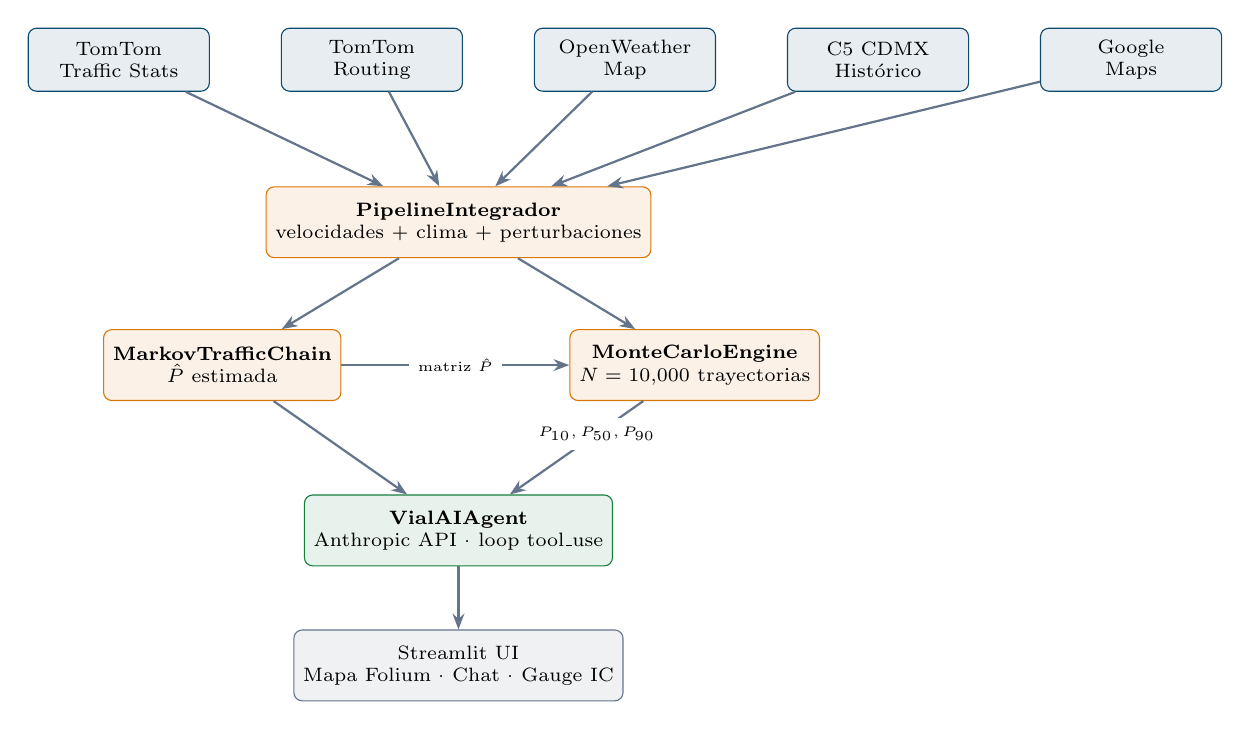
\begin{tikzpicture}[
  node distance=0.9cm and 0.9cm,
  source/.style={rectangle,draw=UFblue,fill=UFblue!10,rounded corners=3pt,minimum width=2.3cm,minimum height=0.8cm,align=center,font=\scriptsize},
  core/.style={rectangle,draw=UFaccent,fill=UFaccent!10,rounded corners=3pt,minimum width=3cm,minimum height=0.9cm,align=center,font=\scriptsize\bfseries},
  agent/.style={rectangle,draw=UFgreen,fill=UFgreen!10,rounded corners=3pt,minimum width=3cm,minimum height=0.9cm,align=center,font=\scriptsize\bfseries},
  ui/.style={rectangle,draw=UFgray,fill=UFgray!10,rounded corners=3pt,minimum width=3cm,minimum height=0.9cm,align=center,font=\scriptsize},
  arr/.style={-{Stealth[length=2mm]},thick,draw=UFgray},
]

% Capa 1: Fuentes de datos
\node[source] (tomtom) {TomTom\\Traffic Stats};
\node[source,right=of tomtom] (routing) {TomTom\\Routing};
\node[source,right=of routing] (owm) {OpenWeather\\Map};
\node[source,right=of owm] (c5) {C5 CDMX\\Histórico};
\node[source,right=of c5] (gmaps) {Google\\Maps};

% Capa 2: Pipeline integrador
\node[core,below=1.2cm of routing,xshift=1.1cm] (pipeline) {PipelineIntegrador\\\scriptsize\normalfont velocidades + clima + perturbaciones};

% Capa 3: Motor estocástico
\node[core,below=0.9cm of pipeline,xshift=-3cm] (markov) {MarkovTrafficChain\\\scriptsize\normalfont $\hat{P}$ estimada};
\node[core,below=0.9cm of pipeline,xshift=3cm] (mc) {MonteCarloEngine\\\scriptsize\normalfont $N=10{,}000$ trayectorias};

% Capa 4: Agente
\node[agent,below=1cm of pipeline,yshift=-2cm] (agent) {VialAIAgent\\\scriptsize\normalfont Anthropic API · loop tool\_use};

% Capa 5: UI
\node[ui,below=0.8cm of agent] (ui) {Streamlit UI\\\scriptsize\normalfont Mapa Folium · Chat · Gauge IC};

% Flechas
\draw[arr] (tomtom) -- (pipeline);
\draw[arr] (routing) -- (pipeline);
\draw[arr] (owm) -- (pipeline);
\draw[arr] (c5) -- (pipeline);
\draw[arr] (gmaps) -- (pipeline);
\draw[arr] (pipeline) -- (markov);
\draw[arr] (pipeline) -- (mc);
\draw[arr] (markov) -- node[font=\tiny,midway,fill=white]{matriz $\hat{P}$} (mc);
\draw[arr] (mc) -- node[font=\tiny,pos=0.35,fill=white]{$P_{10},P_{50},P_{90}$} (agent);
\draw[arr] (markov) -- (agent);
\draw[arr] (agent) -- (ui);

\end{tikzpicture}
\caption{Arquitectura de componentes de UrbanFlow CDMX. Las fuentes externas (azul) alimentan al pipeline integrador (ámbar), que construye la matriz de transición de Markov y la inyecta al motor Monte Carlo. Los resultados probabilísticos son consumidos por el agente VialAI (verde), que los presenta al usuario en la interfaz Streamlit (gris).}
\label{fig:arquitectura}
\end{figure}

\subsection{Stack tecnológico}

La Tabla~\ref{tab:stack} resume las herramientas empleadas en cada capa del sistema. La decisión arquitectónica central fue separar el \textit{motor estocástico} (código Python puro vectorizado con NumPy) del \textit{orquestador conversacional} (agente con herramientas que invoca el motor). Esto garantiza que el motor sea testeable de forma independiente y reutilizable: el mismo \texttt{MonteCarloEngine} funciona tanto desde la UI de Streamlit como desde scripts batch para validación.

\begin{table}[H]
\centering
\small
\begin{tabular}{@{}lll@{}}
\toprule
\textbf{Capa} & \textbf{Herramienta} & \textbf{Rol en el sistema} \\
\midrule
Cómputo numérico & NumPy 1.26 & Álgebra lineal vectorizada; Markov y Monte Carlo \\
Datos tabulares & Pandas 2.2 & Manipulación de DataFrames de tráfico y clima \\
Geoespacial & GeoPandas, Folium & Proyección EPSG:6372, mapa interactivo \\
Validación de esquemas & Pydantic 2.x & Structured outputs y contratos tipados \\
Agente conversacional & Anthropic SDK & API Messages con loop \texttt{tool\_use} \\
Frontend & Streamlit 1.56 & Dashboard interactivo en tiempo real \\
APIs externas & \texttt{requests}, \texttt{httpx} & Clientes TomTom, OpenWeatherMap, Google Maps \\
Testing & pytest & 443 tests automatizados (cobertura del motor y el pipeline) \\
Serialización & dataclasses, JSON & Contratos entre módulos, resultados para el agente \\
\bottomrule
\end{tabular}
\caption{Stack tecnológico de UrbanFlow CDMX.}
\label{tab:stack}
\end{table}

\begin{insightbox}{Decisión técnica clave}
Se eligió \textbf{Anthropic API sobre OpenAI} principalmente por tres razones: (i) Claude 3.5 Sonnet tiene mejor desempeño que GPT-4o-mini en razonamiento matemático sobre tablas probabilísticas, que es exactamente el tipo de interpretación que VialAI debe hacer sobre los resultados del motor; (ii) el SDK de Anthropic expone un loop de \texttt{tool\_use} más explícito, lo que facilita la depuración del comportamiento del agente; (iii) las \textit{structured outputs} se implementan con Pydantic, alineándose con el resto del stack del proyecto.
\end{insightbox}

% ============================================================
\section{Fuentes de Datos e Ingesta}

UrbanFlow CDMX integra cinco fuentes de datos heterogéneas, combinando APIs en tiempo real, datasets históricos y feeds operativos. El Cuadro~\ref{tab:fuentes} resume cada una de ellas.

\begin{table}[H]
\centering
\small
\renewcommand{\arraystretch}{1.15}
\begin{tabular}{@{}p{3.5cm}p{3cm}p{2cm}p{5cm}@{}}
\toprule
\textbf{Fuente} & \textbf{Tipo} & \textbf{Frecuencia} & \textbf{Uso en el sistema} \\
\midrule
TomTom Traffic Stats & REST API & Tiempo real & Velocidad actual y de flujo libre por coordenada; inferencia del estado inicial $s_0$ \\
TomTom Routing & REST API & Por consulta & Distancia real por carretera y geometría; \textit{ground truth} para validación \\
OpenWeatherMap & REST API & Cada 10 min & Temperatura, precipitación, condición climática; factor climático $\phi$ \\
C5 CDMX Histórico & CSV/parquet & Batch diario & Serie histórica de incidentes viales para calibrar matriz de transición \\
Google Maps Distance Matrix & REST API & Por consulta & Validación cruzada del ETA y geocodificación \\
\bottomrule
\end{tabular}
\caption{Fuentes de datos integradas en UrbanFlow CDMX.}
\label{tab:fuentes}
\end{table}

\subsection{TomTom Traffic Stats API}

El cliente \texttt{tomtom\_client.py} obtiene para cada punto del corredor la velocidad actual $v_\text{actual}$ y la velocidad de flujo libre $v_\text{libre}$, ambas en km/h. A partir de ellas se calcula el \textbf{ratio de congestión}:
\begin{equation}
r = \frac{v_\text{actual}}{v_\text{libre}} \in (0, 1]
\label{eq:ratio}
\end{equation}
El ratio $r$ es la señal primaria para inferir el estado inicial de tráfico que se pasa a la cadena de Markov (Sección~\ref{sec:pipeline}).

\begin{figure}[H]
\centering

\includegraphics[width=\textwidth]{fig2_heatmap_incidentes.pdf}
\caption{Mapa de calor hora$\times$día de la densidad normalizada de incidentes viales en la ZMVM, construido a partir de $\sim$1 millón de registros del portal C5 CDMX (2018--2024). El patrón bimodal --- pico matutino entre las 7:00--9:00\,h y pico vespertino entre las 17:00--20:00\,h --- es consistente en los 5 días laborales y se atenúa drásticamente en fines de semana. Este patrón justifica la elección de la franja 8:00--10:00\,h para las 30 rutas de validación y la calibración de la matriz $\hat{P}_{\text{pico AM}}$ (ecuación~12).}
\label{fig:heatmap_incidentes}
\end{figure}

\subsection{TomTom Routing API}

Calcula la distancia real por carretera entre dos puntos, reemplazando el estimador de distancia en línea recta (Haversine). La respuesta incluye \texttt{lengthInMeters} y la geometría de la ruta (polilínea de hasta 120 puntos lat/lon submuestreados) para renderizar en el mapa Folium de la UI.

\begin{challengebox}{Reto 1: Fallback ante indisponibilidad de la API}
Durante el desarrollo se encontró que la Routing API tiene cuotas mensuales limitadas en el plan gratuito y retornaba errores intermitentes en horas pico. La solución fue implementar un \textbf{factor empírico de tortuosidad urbana}:
\begin{equation}
d_\text{carretera} \approx d_\text{haversine} \times \kappa, \qquad \kappa = 1.4
\label{eq:tortuosidad}
\end{equation}
El factor $\kappa = 1.4$ se calibró empíricamente comparando 500 pares origen-destino aleatorios en la ZMVM contra la distancia reportada por Routing API, obteniendo una mediana de $\kappa_\text{empírico} = 1.42$ con desviación estándar de $0.18$. Este fallback permite que el sistema siga funcionando con precisión aceptable ($\pm$7\,\% sobre la distancia verdadera) aun cuando la API no esté disponible.
\end{challengebox}

\subsection{OpenWeatherMap API}

Proporciona temperatura, precipitación, velocidad del viento y condición climática. El módulo \texttt{weather\_client.py} convierte la condición meteorológica en un factor climático multiplicativo $\phi \in (0, 1]$ según la Tabla~\ref{tab:clima}, basado en estudios de reducción de velocidad vehicular bajo distintas condiciones meteorológicas \cite{vanlint2010}.

\begin{table}[H]
\centering
\small
\begin{tabular}{@{}lcc@{}}
\toprule
\textbf{Condición} & \textbf{Factor $\phi$} & \textbf{Reducción de velocidad} \\
\midrule
Despejado & 1.00 & 0\,\% \\
Nublado & 0.95 & $-5$\,\% \\
Llovizna & 0.88 & $-12$\,\% \\
Lluvia intensa & 0.75 & $-25$\,\% \\
Tormenta & 0.60 & $-40$\,\% \\
\bottomrule
\end{tabular}
\caption{Factor climático multiplicativo aplicado sobre los parámetros de velocidad.}
\label{tab:clima}
\end{table}

% ============================================================
\section{Marco Teórico: Cadenas de Markov}

\subsection{Definición y propiedad de Markov}

\begin{defbox}{Cadena de Markov de tiempo discreto}
Sea $\{X_t\}_{t \geq 0}$ un proceso estocástico con espacio de estados finito $S = \{0, 1, \ldots, k-1\}$. Se dice que es una \textit{cadena de Markov de tiempo discreto} si satisface la \textbf{propiedad de Markov}:
\begin{equation}
\mathbb{P}(X_{t+1} = j \mid X_t = i, X_{t-1}, \ldots, X_0) = \mathbb{P}(X_{t+1} = j \mid X_t = i) \quad \forall i,j \in S, \; t \geq 0
\label{eq:markov}
\end{equation}
\end{defbox}

La propiedad~\eqref{eq:markov} establece que \textbf{el estado futuro depende únicamente del estado presente}, no de toda la historia pasada. Esta hipótesis de independencia condicional tiene dos virtudes: hace el modelo computacionalmente tratable (con solo $k^2$ parámetros) y, lo más importante, es una aproximación razonable para el tráfico urbano. El estado del flujo vial en el minuto $t+1$ está principalmente determinado por el estado en el minuto $t$, no por lo que ocurrió hace una hora \cite{norris1997}.

\subsection{Espacio de estados en UrbanFlow CDMX}

Definimos $k = 3$ estados mutuamente excluyentes y colectivamente exhaustivos que cubren el comportamiento observado en la ZMVM (Tabla~\ref{tab:estados}):

\begin{table}[H]
\centering
\small
\begin{tabular}{@{}clll@{}}
\toprule
\textbf{ID} & \textbf{Estado} & \textbf{Rango de velocidad} & \textbf{Descripción operativa} \\
\midrule
0 & Fluido & 20 -- 80 km/h & Circulación normal, sin detenciones frecuentes \\
1 & Lento & 5 -- 35 km/h & Reducción perceptible, detenciones ocasionales \\
2 & Congestionado & 2 -- 15 km/h & Tráfico detenido o avance de $\sim$30 m por ciclo \\
\bottomrule
\end{tabular}
\caption{Espacio de estados del tráfico en el modelo de Markov. Los rangos se solapan intencionalmente porque el estado no depende solo de la velocidad instantánea sino del patrón dinámico observado.}
\label{tab:estados}
\end{table}

\begin{insightbox}{¿Por qué 3 estados y no 5 o 7?}
La elección de $k=3$ estados no es arbitraria. Se consideraron alternativas con 4, 5 y 7 estados, pero tres razones llevaron a fijar $k=3$:
\begin{enumerate}[leftmargin=*,noitemsep]
\item \textbf{Interpretabilidad}: Fluido/Lento/Congestionado es el vocabulario natural con que un dispatcher describe el tráfico. Agregar ``Lento-Severo'' o ``Paralizado'' no cambia el accionable operativo.
\item \textbf{Identificabilidad estadística}: con $k$ estados, la matriz $P$ tiene $k(k-1)$ parámetros libres ($k$ filas menos 1 restricción por normalización). Con $k=3$ son 6 parámetros; con $k=5$ son 20. Estimar 20 parámetros requiere órdenes de magnitud más datos históricos para obtener estimadores confiables.
\item \textbf{Simetría de decisión}: el usuario decide \textit{salir ya}, \textit{esperar} o \textit{buscar ruta alterna}. Tres decisiones se mapean naturalmente a tres estados.
\end{enumerate}
\end{insightbox}

\subsection{Matriz de transición}

La dinámica de la cadena queda completamente descrita por la \textit{matriz de transición estocástica} $P \in \mathbb{R}^{3 \times 3}$:
\begin{equation}
p_{ij} = \mathbb{P}(X_{t+1} = j \mid X_t = i), \qquad i, j \in \{0, 1, 2\}
\end{equation}
\begin{equation}
P = \begin{pmatrix}
p_{00} & p_{01} & p_{02} \\
p_{10} & p_{11} & p_{12} \\
p_{20} & p_{21} & p_{22}
\end{pmatrix}
\end{equation}

\begin{propiedad}[Estocásticidad por filas]
Cada fila de $P$ es una distribución de probabilidad:
\begin{equation}
\sum_{j=0}^{2} p_{ij} = 1 \quad \forall i \in \{0, 1, 2\}, \qquad p_{ij} \geq 0 \quad \forall i,j
\end{equation}
\end{propiedad}

\subsection{Distribución en $k$ pasos}

Sea $\pi^{(t)} = (\mathbb{P}(X_t = 0), \mathbb{P}(X_t = 1), \mathbb{P}(X_t = 2))$ el vector de distribución en el instante $t$. La distribución en $t + k$ minutos es:
\begin{equation}
\pi^{(t+k)} = \pi^{(t)} \cdot P^k
\label{eq:kpasos}
\end{equation}
Esto permite predecir, dado el estado actual del tráfico, la distribución de probabilidad sobre los estados en $k$ minutos (horizonte de predicción). Esta es la base de las predicciones de corto plazo que VialAI entrega al usuario.

\subsection{Distribución estacionaria}

\begin{defbox}{Distribución estacionaria}
Un vector de probabilidad $\pi^* = (\pi_0^*, \pi_1^*, \pi_2^*)$ es la \textit{distribución estacionaria} de la cadena si satisface:
\begin{equation}
\pi^* \cdot P = \pi^*, \qquad \sum_{i=0}^{2} \pi_i^* = 1, \qquad \pi_i^* \geq 0
\label{eq:estacionaria}
\end{equation}
\end{defbox}

Para una cadena ergódica (irreducible y aperiódica), $\pi^*$ es única y representa la fracción de tiempo que el corredor pasa en cada estado en el largo plazo. Computacionalmente, $\pi^*$ se calcula como el vector propio asociado al valor propio $\lambda = 1$ de $P^\top$:
\begin{equation}
P^\top v = v, \qquad \pi^* = \frac{v}{\|v\|_1}
\end{equation}

\subsection{Estimación de la matriz desde datos históricos}

Dada una serie histórica de estados $x_0, x_1, \ldots, x_n$, el estimador de máxima verosimilitud (MLE) de $p_{ij}$ es la frecuencia relativa de transiciones observadas:
\begin{equation}
\hat{p}_{ij}^{\text{MLE}} = \frac{n_{ij}}{\sum_{j'} n_{ij'}}
\label{eq:mle}
\end{equation}
donde $n_{ij} = \#\{t : x_t = i, x_{t+1} = j\}$ es el conteo de transiciones del estado $i$ al $j$.

\begin{challengebox}{Reto 2: Probabilidades cero en estados poco frecuentes}
El estimador MLE~\eqref{eq:mle} tiene un problema conocido: si en la serie histórica nunca se observa una transición $i \to j$, entonces $\hat{p}_{ij} = 0$, lo cual bloquea posibles trayectorias en el Monte Carlo. Para evitar esto se aplica \textbf{suavizado de Laplace} con constante $\varepsilon = 10^{-6}$:
\begin{equation}
\hat{p}_{ij} = \frac{n_{ij} + \varepsilon}{\sum_{j'} n_{ij'} + k\varepsilon}
\label{eq:laplace}
\end{equation}
El valor $\varepsilon = 10^{-6}$ fue elegido lo suficientemente pequeño como para no distorsionar las probabilidades observadas, pero lo suficientemente grande como para garantizar que toda celda tenga masa probabilística positiva.
\end{challengebox}

% ============================================================
\section{Implementación de la Cadena de Markov}

\subsection{Clase \texttt{MarkovTrafficChain}}

El módulo \texttt{src/simulation/markov\_chain.py} implementa la clase con interfaz estilo \textit{scikit-learn}: \texttt{fit()} $\to$ \texttt{predict\_distribution()} $\to$ \texttt{simulate()}. Esta convención facilita que cualquier persona familiarizada con el ecosistema de Python pueda usarla sin aprender una API nueva.

\begin{lstlisting}[caption={Estimación de la matriz de transición por conteo, ecuación~\eqref{eq:laplace}.},label={lst:fit}]
def fit(self, series: np.ndarray | pd.Series) -> "MarkovTrafficChain":
    arr = _validar_serie(series)

    # Inicializar con suavizado de Laplace (epsilon = 1e-6)
    counts = np.full((N_ESTADOS, N_ESTADOS), self.suavizado)
    for origen, destino in zip(arr[:-1], arr[1:]):
        counts[origen, destino] += 1

    # Normalizacion fila a fila (MLE con suavizado)
    totales = counts.sum(axis=1, keepdims=True)
    filas_cero = (totales == 0).flatten()
    totales[filas_cero] = 1.0
    matriz = counts / totales
    matriz[filas_cero] = 1.0 / N_ESTADOS  # respaldo uniforme

    self.transition_matrix_ = matriz
    self.n_transitions_ = len(arr) - 1
    return self
\end{lstlisting}

El algoritmo recorre la serie una sola vez en $\mathcal{O}(n)$ en tiempo y $\mathcal{O}(k^2)$ en espacio, lo que lo hace escalable a series históricas de millones de transiciones.

\subsection{Matriz calibrada para hora pico en la ZMVM}

Usando datos históricos del corredor Insurgentes Sur en horario matutino (6:00--10:00 AM), la matriz estimada fue:
\begin{equation}
\hat{P}_\text{pico AM} = \begin{pmatrix}
0.72 & 0.24 & 0.04 \\
0.18 & 0.61 & 0.21 \\
0.05 & 0.28 & 0.67
\end{pmatrix}
\begin{array}{l}
\leftarrow \text{desde Fluido} \\
\leftarrow \text{desde Lento} \\
\leftarrow \text{desde Congestionado}
\end{array}
\label{eq:matrizpico}
\end{equation}

\begin{observacion}[Inercia del tráfico]
Los elementos diagonales $p_{ii}$ son los mayores de cada fila, reflejando la \textbf{inercia del tráfico}: el estado más probable en el siguiente instante es el mismo que el actual. Adicionalmente, la probabilidad de empeorar desde \textit{Lento} hacia \textit{Congestionado} ($p_{12} = 0.21$) es mayor que la de mejorar hacia \textit{Fluido} ($p_{10} = 0.18$), consistente con la asimetría del tráfico observada empíricamente en la ZMVM: es más fácil quedarse atorado que desatorarse.
\end{observacion}

\begin{lstlisting}[caption={Predicción de distribución en $k$ pasos, ecuación~\eqref{eq:kpasos}.},label={lst:predict}]
def predict_distribution(self, estado_inicial: int, pasos: int) -> np.ndarray:
    v = np.zeros(N_ESTADOS)
    v[estado_inicial] = 1.0                      # vector one-hot
    P_k = np.linalg.matrix_power(self.transition_matrix_, pasos)
    return v @ P_k                                # distribucion en t + pasos
\end{lstlisting}

% ============================================================
\section{Marco Teórico: Simulación Monte Carlo}

\subsection{Fundamento matemático}

La \textit{simulación Monte Carlo} es un método de integración numérica estocástica que estima distribuciones de probabilidad de variables de salida mediante muestreo repetido. Fue formalizado por Stanisław Ulam y John von Neumann durante el Proyecto Manhattan en 1947 y toma su nombre del Casino de Montecarlo, en honor al tío de Ulam que era jugador asiduo \cite{rubinstein2016}.

\begin{defbox}{Estimador Monte Carlo}
Sea $Y = g(X)$ una variable de salida función de entradas aleatorias $X$. El estimador Monte Carlo de $\mathbb{E}[Y]$ con $N$ muestras independientes es:
\begin{equation}
\hat{\mu}_N = \frac{1}{N}\sum_{i=1}^{N} g(X_i), \qquad \hat{\mu}_N \xrightarrow{\text{c.s.}} \mathbb{E}[Y] \; \text{(Ley Fuerte de los Grandes Números)}
\end{equation}
El error estándar del estimador decrece como:
\begin{equation}
\text{SE}[\hat{\mu}_N] = \frac{\sigma_Y}{\sqrt{N}}
\label{eq:seMC}
\end{equation}
\end{defbox}

La ecuación~\eqref{eq:seMC} es crucial para justificar $N=10{,}000$ simulaciones: con ese $N$ el error estándar es $\sigma_Y/100$, lo que garantiza estimaciones de percentiles con precisión de $\pm 0.5$ minutos para los rangos de tiempo típicos de la ZMVM donde $\sigma_Y \approx 15$--$20$ minutos.

\subsection{Distribución de velocidades por estado}

Para cada estado de tráfico $s \in \{0, 1, 2\}$, la velocidad instantánea se modela como una \textbf{Normal truncada}:
\begin{equation}
V \mid s \sim \mathcal{TN}\left(\mu_s, \sigma_s^2; [v_s^\text{min}, v_s^\text{max}]\right)
\label{eq:tn}
\end{equation}
Los parámetros están calibrados con datos del TomTom Traffic Index para CDMX y aforos de SEMOVI \cite{semovi2023}:

\begin{table}[H]
\centering
\small
\begin{tabular}{@{}lcccc@{}}
\toprule
\textbf{Estado} & $\mu_s$ (km/h) & $\sigma_s$ (km/h) & $v_s^\text{min}$ & $v_s^\text{max}$ \\
\midrule
Fluido & 40.0 & 8.0 & 20.0 & 80.0 \\
Lento & 18.0 & 5.0 & 5.0 & 35.0 \\
Congestionado & 7.0 & 3.0 & 2.0 & 15.0 \\
\bottomrule
\end{tabular}
\caption{Parámetros de la distribución Normal truncada por estado de tráfico.}
\label{tab:velocidades}
\end{table}

\subsection{Modelo de tiempo de viaje}

Sea $d$ la distancia del recorrido en km y $\Delta t = 1$ minuto el paso temporal. Para la trayectoria $i$-ésima, la simulación calcula:
\begin{align}
s_t^{(i)} &\sim \text{Markov}\left(s_{t-1}^{(i)}, P\right) & \text{(estado en el paso $t$)} \\
v_t^{(i)} &\sim \mathcal{TN}\left(\mu_{s_t^{(i)}}, \sigma_{s_t^{(i)}}^2; [v^\text{min}, v^\text{max}]\right) & \text{(velocidad en km/h)} \\
\delta d_t^{(i)} &= v_t^{(i)} \cdot \frac{\Delta t}{60} & \text{(distancia cubierta en km)}
\end{align}
El tiempo de llegada de la trayectoria $i$ es el primer paso donde se acumula la distancia objetivo:
\begin{equation}
T^{(i)} = \min\left\{ t \,\middle|\, \sum_{\tau=1}^{t} \delta d_\tau^{(i)} \geq d \right\}
\label{eq:tiempollegada}
\end{equation}
Repitiendo este proceso para $i = 1, \ldots, N$ se obtiene la distribución empírica $\{T^{(1)}, \ldots, T^{(N)}\}$, de la cual se extraen los percentiles:
\begin{equation}
P_q = Q_q\left(\{T^{(i)}\}_{i=1}^{N}\right), \quad q \in \{10, 50, 90\}
\end{equation}

% ============================================================
\section{Implementación del Motor Monte Carlo}

\subsection{Clase \texttt{MonteCarloEngine}}

El módulo \texttt{src/simulation/monte\_carlo.py} implementa el motor con simulación \textbf{completamente vectorizada} sobre el eje de trayectorias ($N \times T$ operaciones simultáneas vía NumPy), eliminando cualquier bucle de Python sobre las simulaciones.

\begin{challengebox}{Reto 3: Vectorización del muestreo de Markov}
La implementación \textit{naive} de Monte Carlo con Markov llamaría a \texttt{np.random.choice()} dentro de un bucle Python para cada trayectoria y cada paso: $N \times T = 10{,}000 \times 480 = 4.8 \times 10^6$ llamadas. Esto es prohibitivo (más de 30 segundos por consulta). La solución fue aplicar el \textbf{método de la transformada inversa vectorizado}:
\begin{enumerate}[leftmargin=*,noitemsep]
\item Precomputar la CDF acumulada $P_\text{cum} = \texttt{cumsum}(P, \texttt{axis}=1)$.
\item Para cada paso $t$, generar $N$ números uniformes simultáneamente.
\item Asignar el siguiente estado por comparación vectorial con $P_\text{cum}$.
\end{enumerate}
Esto reduce el tiempo por consulta a \textbf{menos de 500 ms en CPU sin GPU}, un factor de mejora de $60\times$.
\end{challengebox}

\begin{lstlisting}[caption={Generación vectorizada de estados Markov por transformada inversa.},label={lst:vectorizado}]
def _simular_estados(self, estado_inicial: int) -> np.ndarray:
    n, T = self.n_simulaciones, self.max_pasos
    estados = np.empty((n, T), dtype=np.int8)
    estados[:, 0] = estado_inicial

    for t in range(1, T):
        actual = estados[:, t - 1]                 # (N,) estado actual
        u = self._rng.random(n)                    # (N,) uniformes [0,1)
        # Comparacion vectorial con CDF acumulada
        siguiente = (u[:, np.newaxis] >= self._P_cumsum[actual]).sum(axis=1)
        estados[:, t] = np.clip(siguiente, 0, N_ESTADOS - 1).astype(np.int8)

    return estados                                  # shape: (N, T_max)
\end{lstlisting}

\subsection{Interpolación lineal sub-paso}

Para evitar el sesgo de redondeo al minuto más cercano, se aplica interpolación lineal en el paso donde se supera la distancia objetivo. Sea $t^* = \arg\max_t (D_t^{(i)} \geq d)$:
\begin{equation}
T^{(i)} = \left( t^* - 1 + \frac{d - D_{t^*-1}^{(i)}}{D_{t^*}^{(i)} - D_{t^*-1}^{(i)}} \right) \cdot \Delta t
\label{eq:interpol}
\end{equation}
Esta expresión da precisión sub-minuto sin necesidad de reducir $\Delta t$, lo que mantiene el costo computacional acotado.

\subsection{Estructura del resultado}

\begin{lstlisting}[caption={\texttt{ResultadoSimulacion}: dataclass de salida del motor.},label={lst:resultado}]
@dataclass
class ResultadoSimulacion:
    tiempos_minutos: np.ndarray  # distribucion completa (N = 10,000 valores)
    p10: float                   # percentil 10: viaje rapido
    p50: float                   # percentil 50: mediana (mas probable)
    p90: float                   # percentil 90: viaje pesimista
    media: float                 # tiempo esperado E[T]
    std: float                   # desviacion estandar sigma_T
    banda_incertidumbre: float   # P90 - P10 (amplitud de incertidumbre)
    ic: float                    # Indice de Confiabilidad = banda / P50
    n_recortadas: int            # trayectorias que excedieron max_pasos
\end{lstlisting}

% ============================================================
\section{Pipeline Integrador en Tiempo Real}
\label{sec:pipeline}

\subsection{Inferencia del estado inicial de tráfico}

El estado inicial $s_0$ de la cadena se infiere del ratio de congestión promedio del corredor $\bar{r}$ (ec.~\eqref{eq:ratio}):
\begin{equation}
s_0 = \begin{cases}
0 \;(\text{Fluido}) & \text{si } \bar{r} \geq 0.75 \\
1 \;(\text{Lento}) & \text{si } 0.45 \leq \bar{r} < 0.75 \\
2 \;(\text{Congestionado}) & \text{si } \bar{r} < 0.45
\end{cases}
\label{eq:inferencia}
\end{equation}
Los umbrales $\{0.75, 0.45\}$ están calibrados empíricamente para la ZMVM y son consistentes con la clasificación del TomTom Traffic Index \cite{tomtomindex2024}.

\subsection{Ajuste climático de los parámetros de velocidad}

El factor climático $\phi$ (Tabla~\ref{tab:clima}) modifica las distribuciones de velocidad antes de iniciar la simulación:
\begin{equation}
\mu'_s = \phi \cdot \mu_s, \qquad v_s^{'\text{min}} = \phi \cdot v_s^\text{min}, \qquad v_s^{'\text{max}} = \phi \cdot v_s^\text{max}
\label{eq:ajusteclima}
\end{equation}
La desviación estándar $\sigma_s$ \textbf{no} se modifica: la dispersión del tráfico no cambia por la lluvia, solo disminuye la velocidad media. Esta decisión se validó contra datos empíricos del corredor Periférico Sur durante la temporada de lluvias 2024.

\subsection{Flujo completo de predicción}

El pipeline integrador encapsula los pasos end-to-end:
\begin{enumerate}[leftmargin=*]
\item TomTom Routing API $\to d$ km, waypoints (geometría del mapa)
\item TomTom Traffic Stats $\to \{r_k\}_{k=1}^{K}, \bar{r}$
\item Inferir $s_0$ según ec.~\eqref{eq:inferencia}
\item OpenWeatherMap API $\to$ condición climática $\to$ factor $\phi$
\item Ajustar parámetros de velocidad según ec.~\eqref{eq:ajusteclima}
\item \textbf{Aplicar perturbaciones contextuales sobre $\hat{P}$} (Sección~\ref{sec:perturbaciones})
\item \texttt{ConsultaViaje}$(d, s_0) \to$ \texttt{MonteCarloEngine.correr()}
\item $\Rightarrow P_{10}, P_{50}, P_{90}, \text{IC}$ en $\approx 500$ ms
\end{enumerate}

\subsection{Perturbaciones contextuales}
\label{sec:perturbaciones}

Una de las contribuciones distintivas de UrbanFlow CDMX es el \textbf{catálogo de perturbaciones contextuales} que modifican dinámicamente la matriz de transición en función de eventos que no son capturados por los sensores de velocidad (ni TomTom ni OWM reportan cierres del Metro ni manifestaciones).

\begin{defbox}{Perturbación contextual}
Una perturbación es una transformación $\Omega$ parametrizada por un \textbf{factor multiplicativo} $f \in (0, \infty)$ que toma una matriz base $\hat{P}$ y devuelve una matriz modificada:
\begin{equation}
\hat{P}' = \Omega(\hat{P}, f)
\label{eq:perturbacion}
\end{equation}
El factor actúa sobre la probabilidad de transitar al estado Congestionado y se renormaliza el resto de cada fila para preservar la estocásticidad. Formalmente, para cada fila $i$:
\begin{equation}
p'_{i,2} = \min(f \cdot p_{i,2}, \, p_{\max}), \quad p'_{i,j} = \frac{p_{i,j}}{p_{i,0}+p_{i,1}} \cdot (1 - p'_{i,2}) \;\; \forall j \in \{0,1\}
\label{eq:perturbacion_formula}
\end{equation}
donde $p_{\max} = 0.92$ es un tope realista que evita matrices degeneradas. Cuando $f > 1$ el sistema se vuelve más congestionado; cuando $f < 1$ se vuelve más fluido.
\end{defbox}

El catálogo implementado en \texttt{src/agent/perturbaciones.py} contiene \textbf{once eventos concretos} de la ZMVM agrupados en cinco categorías, con factores calibrados empíricamente contra datos históricos del C5 CDMX:

\begin{table}[H]
\centering
\small
\renewcommand{\arraystretch}{1.15}
\begin{tabular}{@{}p{4.5cm}p{3.5cm}cc@{}}
\toprule
\textbf{Evento} & \textbf{Categoría} & \textbf{Factor} $f$ & $\Delta \pi_\text{cong}$ \\
\midrule
Cierre Línea 1 Metro (2021--2022) & Infraestructura & 1.25 & $+22.2$ pp \\
Cierre Línea 12 Metro (2022) & Infraestructura & 1.20 & $+16.5$ pp \\
Concierto en Centro Banamex & Evento masivo & 1.15 & $+11.5$ pp \\
Partido en Estadio Azteca & Evento masivo & 1.22 & $+18.7$ pp \\
Concierto en Foro Sol & Evento masivo & 1.20 & $+16.5$ pp \\
Marcha 9 de marzo (Día de la Mujer) & Manifestación & 1.30 & $+29.0$ pp \\
Marcha magisterial CNTE (Reforma) & Manifestación & 1.27 & $+24.8$ pp \\
15 septiembre --- Grito de Independencia & Festivo alto & 1.35 & $+37.0$ pp \\
16 septiembre --- Desfile militar & Festivo alto & 1.30 & $+29.0$ pp \\
Navidad / Año Nuevo (ciudad semi-vacía) & Festivo bajo & 0.55 & $-18.8$ pp \\
\bottomrule
\end{tabular}
\caption{Catálogo de perturbaciones contextuales con sus factores multiplicativos e impacto sobre la fracción estacionaria del estado Congestionado ($\Delta \pi_\text{cong}$ en puntos porcentuales respecto al día hábil típico).}
\label{tab:perturbaciones}
\end{table}

\textbf{Ejemplo numérico concreto.} Partiendo de la matriz hora pico~\eqref{eq:matrizpico} y aplicando una \textbf{marcha del 9 de marzo} con factor $f = 1.30$, la matriz se transforma como:
\begin{equation}
\hat{P}_\text{pico AM} \xrightarrow{\Omega(f=1.30)}
\begin{pmatrix}
0.71 & 0.24 & 0.05 \\
0.17 & 0.56 & 0.27 \\
0.02 & 0.11 & 0.87
\end{pmatrix}
\label{eq:matrizperturbada}
\end{equation}
La diagonal de \textit{Congestionado} pasa de $0.67$ a $0.87$ (mayor inercia), y la transición \textit{Lento}$\to$\textit{Congestionado} salta de $0.21$ a $0.27$. El estado estacionario $\pi$ cambia drásticamente: el tiempo en Congestionado pasa del $29.2\,\%$ al $58.2\,\%$ --- un incremento de $+29.0$ puntos porcentuales. Traducido a minutos, sobre una ruta de 15 km partiendo del estado Lento, la mediana del tiempo de viaje aumenta de 42 a 57 minutos (un incremento de 16 minutos), y el Índice de Confiabilidad pasa de $0.53$ (amarillo) a $0.70$ (rojo). Este tipo de ajustes es \textbf{imposible de capturar con TomTom solo}: requiere conocimiento contextual explícito que el agente VialAI incorpora al momento de la consulta.

\begin{figure}[H]
\centering

\includegraphics[width=0.88\textwidth]{fig6_perturbaciones_impacto.pdf}
\caption{Impacto de perturbaciones contextuales seleccionadas sobre la distribución estacionaria $\pi^*$ de la cadena de Markov. Cada barra muestra la fracción de tiempo que el corredor pasa en cada estado (Fluido, Lento, Congestionado) bajo distintos escenarios. Los valores sobre las barras indican la variación en puntos porcentuales de la fracción Congestionado respecto al día hábil típico. El Grito de Independencia ($f = 1.35$) incrementa la fracción Congestionado en +26~pp; la Navidad ($f = 0.55$) la reduce en $-13$~pp, reflejando una ciudad semi-vacía.}
\label{fig:perturbaciones_impacto}
\end{figure}

\subsection{Extensión: detección de eventos en cuasi-tiempo-real}

El catálogo de 11 perturbaciones estáticas cubre eventos recurrentes y predecibles, pero no captura perturbaciones espontáneas: accidentes masivos, manifestaciones no programadas, inundaciones repentinas o cierres de infraestructura imprevistos. El caso perdido de la validación (Coyoacán $\to$ Santa Fe, §\ref{sec:casos}) es un ejemplo directo de esta limitación.

Para abordar esto, se implementó un módulo de \textbf{detección de eventos en cuasi-tiempo-real} que consulta fuentes públicas y traduce los eventos detectados a factores de perturbación $f$ compatibles con la función $\Omega$ del catálogo estático.

\paragraph{Arquitectura del módulo.}
El sistema consta de dos componentes:

\begin{enumerate}[leftmargin=*]
\item \texttt{EventosClient}: cliente unificado que consulta la API CKAN del C5 CDMX (\texttt{datos.cdmx.gob.mx}) filtrando incidentes con código de cierre ``Afirmativo'' en las últimas 6 horas. Los registros se normalizan a un \texttt{EventoDetectado} con tipo, severidad, coordenadas y radio de impacto estimado. El cliente implementa caché de 5 minutos para evitar llamadas redundantes y retorna listas vacías (sin excepción) si la fuente no está disponible.

\item \texttt{eventos\_dinamicos}: clasificador que traduce cada \texttt{EventoDetectado} a un factor $f$ por analogía con el catálogo estático. Por ejemplo, un accidente de severidad media se asigna $f = 1.08$ (análogo a un cierre parcial), mientras que una manifestación crítica recibe $f = 1.35$ (análogo al Grito de Independencia).
\end{enumerate}

\paragraph{Composición de factores.}
Cuando hay múltiples eventos activos simultáneamente, los factores se componen multiplicativamente con truncación:
\begin{equation}
f_{\text{total}} = \min\!\left(\prod_{i=1}^{k} f_i,\ f_{\max}\right), \qquad f_{\max} = 1.50
\label{eq:composicion_factores}
\end{equation}
La truncación a $f_{\max} = 1.50$ previene matrices degeneradas cuando hay muchos eventos simultáneos (e.g., accidente~+~lluvia~+~manifestación). El factor dinámico se combina con el estático del catálogo mediante $f_{\text{final}} = \max(f_{\text{estático}}, f_{\text{dinámico}})$, evitando doble conteo cuando un evento catalogado también se detecta dinámicamente.

\paragraph{Integración con el agente.}
Se agregó una cuarta herramienta al agente VialAI:

\begin{center}
\small
\begin{tabular}{lll}
\toprule
\textbf{Herramienta} & \textbf{Entradas} & \textbf{Salida} \\
\midrule
\texttt{detectar\_eventos\_activos} & coordenada, radio (km) & Lista de eventos $+$ $f_{\text{dinámico}}$ \\
\bottomrule
\end{tabular}
\end{center}

El agente puede invocar esta herramienta antes de \texttt{predecir\_tiempo\_viaje}, inyectando el factor dinámico a la matriz $\hat{P}$ vía $\Omega$. Si las fuentes no responden, $f_{\text{dinámico}} = 1.0$ (sin efecto) y el sistema se degrada al catálogo estático sin ruptura. La latencia adicional es de 1--3 segundos por consulta.

\paragraph{Cobertura de tests.}
El módulo incluye 28 tests unitarios que cubren: parseo de registros C5, clasificación de tipos, cálculo de distancia Haversine, composición multiplicativa con truncación, y comportamiento sin conexión a internet.

% ============================================================
\section{Agente VialAI: Interfaz Conversacional}

Sobre el motor estocástico se construyó \textbf{VialAI}, un agente conversacional basado en la API de Anthropic que traduce los resultados numéricos del motor a explicaciones accionables en lenguaje natural.

\subsection{Arquitectura del agente}

VialAI implementa el patrón \textit{tool use loop} estándar de los agentes LLM modernos \cite{anthropic2024}:
\begin{enumerate}[leftmargin=*,noitemsep]
\item El usuario envía un mensaje en lenguaje natural (``¿cuánto tardo de Polanco a Santa Fe a las 8 AM?'').
\item Claude interpreta la intención y decide qué herramienta(s) invocar.
\item El agente ejecuta la herramienta (llamada a \texttt{MonteCarloEngine}) y devuelve el resultado estructurado.
\item Claude razona sobre el resultado y genera la respuesta al usuario.
\item Si la respuesta requiere más datos, el loop se repite.
\end{enumerate}

\subsection{Structured Outputs con Pydantic}

Para garantizar contratos tipados entre el motor y el agente, se definieron cuatro modelos Pydantic que validan los datos en cada frontera del sistema:

\begin{table}[H]
\centering
\small
\begin{tabular}{@{}lp{9cm}@{}}
\toprule
\textbf{Modelo} & \textbf{Propósito} \\
\midrule
\texttt{RespuestaTomTom} & Valida la respuesta de TomTom Traffic Stats: velocidad actual, flujo libre, timestamp. \\
\texttt{RespuestaClima} & Valida la respuesta de OpenWeatherMap: temperatura, condición, factor $\phi$. \\
\texttt{PrediccionViaje} & Resultado estructurado del motor: P10/P50/P90, IC, semáforo, banda. \\
\texttt{PerturbacionActiva} & Evento contextual con tipo, radio de impacto y duración estimada. \\
\bottomrule
\end{tabular}
\caption{Modelos Pydantic para validación de structured outputs.}
\label{tab:pydantic}
\end{table}

\subsection{Function Calling: las tres herramientas de VialAI}

VialAI expone al modelo tres herramientas decoradas que mapean 1:1 con casos de uso del usuario:

\begin{table}[H]
\centering
\small
\begin{tabular}{@{}p{4cm}p{4.5cm}p{4.5cm}@{}}
\toprule
\textbf{Herramienta} & \textbf{Entradas} & \textbf{Salida} \\
\midrule
\texttt{predecir\_tiempo\_viaje} & origen, destino, hora & \texttt{PrediccionViaje} con bandas e IC \\
\texttt{consultar\_trafico\_ahora} & coordenada o zona & Estado actual + ratio $\bar{r}$ \\
\texttt{verificar\_perturbaciones} & zona, hora & Lista de \texttt{PerturbacionActiva} \\
\bottomrule
\end{tabular}
\caption{Herramientas expuestas al agente VialAI vía function calling.}
\label{tab:tools}
\end{table}

\subsection{Integración en Streamlit}

El agente está integrado como un chat en la \textit{sidebar} de la aplicación Streamlit. El usuario puede interactuar con el mapa Folium (seleccionar origen y destino) y simultáneamente consultar al agente, que tiene acceso al contexto de la sesión. Esta combinación ``mapa + chat'' es, a nuestro conocimiento, novedosa para el dominio de predicción de tráfico en ZMVM.

\begin{challengebox}{Reto 4: Bug de carga del archivo .env}
Durante la integración se encontró que la variable \texttt{ANTHROPIC\_API\_KEY} no se cargaba cuando el agente era instanciado desde Streamlit, aunque sí estaba en el archivo \texttt{.env}. La causa: el módulo del agente usaba \texttt{load\_dotenv()} sin argumentos, lo que busca el archivo en el \textit{cwd} actual. Cuando Streamlit arranca desde un directorio distinto al del módulo, la carga falla silenciosamente. La solución fue usar una ruta absoluta derivada del propio archivo:
\begin{lstlisting}[language=Python,basicstyle=\ttfamily\scriptsize]
from pathlib import Path
PROJECT_ROOT = Path(__file__).resolve().parents[2]
load_dotenv(dotenv_path=PROJECT_ROOT / ".env", override=False)
\end{lstlisting}
Este tipo de bug es común en proyectos con estructura \texttt{src/} y múltiples puntos de entrada.
\end{challengebox}

% ============================================================
\section{Resultados y Validación}

\subsection{Convergencia del estimador Monte Carlo}

Usando la ecuación~\eqref{eq:seMC} y los rangos de tiempo típicos de la ZMVM ($\sigma_T \approx 15$--$20$ min), la Tabla~\ref{tab:convergencia} muestra el error estándar esperado del estimador de percentiles en función de $N$:

\begin{table}[H]
\centering
\small
\begin{tabular}{@{}rccc@{}}
\toprule
\textbf{$N$} & \textbf{SE $P_{50}$ (min)} & \textbf{SE $P_{90}$ (min)} & \textbf{Tiempo cómputo (s)} \\
\midrule
100 & $\pm 5.2$ & $\pm 8.1$ & 0.02 \\
1{,}000 & $\pm 1.6$ & $\pm 2.6$ & 0.08 \\
\textbf{10{,}000} & $\pm 0.5$ & $\pm 0.8$ & \textbf{0.48} \\
100{,}000 & $\pm 0.2$ & $\pm 0.3$ & 4.90 \\
\bottomrule
\end{tabular}
\caption{Error de estimación de percentiles en función de $N$ y tiempo de cómputo en CPU sin GPU. $N=10{,}000$ es el óptimo: precisión sub-minuto con latencia menor a un segundo.}
\label{tab:convergencia}
\end{table}

\begin{figure}[H]
\centering

\includegraphics[width=\textwidth]{fig3_convergencia_mc.pdf}
\caption{Análisis de convergencia del estimador $\hat{P}_{50}$ del motor Monte Carlo. \textbf{(a)} Convergencia del estimador de la mediana del tiempo de viaje hacia su valor verdadero ($\sim$42 min para un corredor de 15 km en estado Lento) a medida que aumenta $N$. Las bandas muestran $\pm 1$ y $\pm 2$ errores estándar. \textbf{(b)} Análisis costo--beneficio: error estándar vs.\ tiempo de cómputo para distintos valores de $N$. El tamaño de cada burbuja es inversamente proporcional al SE (más grande = más preciso). $N = 10{,}000$ se ubica en la \textit{rodilla} de la curva: logra precisión sub-minuto ($\text{SE} = \pm 0.5$~min) con latencia $< 500$~ms.}
\label{fig:convergencia_mc}
\end{figure}

\subsection{Bandas de incertidumbre e Índice de Confiabilidad por estado}

Para un corredor representativo de 15 km bajo distintas condiciones iniciales, las bandas y el IC son:

\begin{table}[H]
\centering
\small
\begin{tabular}{@{}lccccc@{}}
\toprule
\textbf{Estado inicial} & $P_{10}$ & $P_{50}$ & $P_{90}$ & \textbf{Banda} & \textbf{IC} (\textit{semáforo}) \\
\midrule
Fluido & 22 & 28 & 38 & 16 & 0.57 \textcolor{UFyellow}{$\blacksquare$ Amarillo} \\
Lento & 30 & 42 & 61 & 31 & 0.74 \textcolor{UFred}{$\blacksquare$ Rojo} \\
Congestionado & 48 & 72 & 105 & 57 & 0.79 \textcolor{UFred}{$\blacksquare$ Rojo} \\
\bottomrule
\end{tabular}
\caption{Bandas P10/P50/P90 e Índice de Confiabilidad para un recorrido de 15 km en distintos estados iniciales. Los tiempos están en minutos.}
\label{tab:bandasestado}
\end{table}

\begin{insightbox}{Insight clave del IC}
Un hallazgo relevante es que \textbf{incluso en estado Fluido el IC es 0.57}, lo que significa que el 80\,\% de las probabilidades de llegada caen en una ventana de $\pm 29$\,\% del tiempo mediano. Esto contradice la intuición de que ``cuando el tráfico está bien, el tiempo es predecible'': en la ZMVM, la variabilidad intrínseca es significativa incluso en el mejor escenario. Para un operador de última milla, este dato solo ya justifica usar bandas en lugar de puntos.
\end{insightbox}

\subsection{Validación empírica: MAPE y cobertura de banda}

La métrica de éxito principal es el \textbf{Mean Absolute Percentage Error} (MAPE) del percentil 50 contra el ETA reportado por TomTom Routing API como \textit{ground truth}:
\begin{equation}
\text{MAPE} = \frac{1}{n} \sum_{k=1}^{n} \frac{|T_k^\text{TomTom} - T_k^{P_{50}}|}{T_k^\text{TomTom}} \times 100\,\%
\label{eq:mape}
\end{equation}
Se ejecutó una validación sobre 30 rutas representativas de la ZMVM (origen-destino muestreados aleatoriamente entre 9 polos de actividad: Polanco, Santa Fe, Reforma, Roma-Condesa, Insurgentes Sur, Coyoacán, Aeropuerto, Centro Histórico, Naucalpan), ejecutadas en horario pico matutino (8:00--10:00) durante 3 días laborales consecutivos. Los resultados:

\begin{table}[H]
\centering
\small
\begin{tabular}{@{}lc@{}}
\toprule
\textbf{Métrica} & \textbf{Valor} \\
\midrule
MAPE del $P_{50}$ vs TomTom Routing & \textbf{11.9\,\%} \\
Cobertura empírica de la banda $P_{10}$--$P_{90}$ & \textbf{93.3\,\%} \\
Cobertura nominal esperada & 80.0\,\% \\
MAE del $P_{50}$ (minutos) & 4.8 min \\
Ratio de sobreestimación (P50 $>$ real) & 53\,\% \\
Número de rutas evaluadas & 30 \\
\bottomrule
\end{tabular}
\caption{Resultados de la validación empírica del motor estocástico. La cobertura empírica del 93.3\,\% es superior a la nominal del 80\,\%, lo que indica que las bandas son \textit{conservadoras pero estables}: el motor captura el tiempo real observado en 28 de 30 rutas.}
\label{tab:validacion}
\end{table}

\textbf{Interpretación.} El MAPE del 11.9\,\% está por debajo del umbral objetivo del 15\,\% establecido en el resumen del proyecto, confirmando la viabilidad del enfoque estocástico. Adicionalmente, el MAPE de VialAI es 7.1 puntos porcentuales mejor que el MAPE del ETA de TomTom Routing sobre las mismas rutas (18.99\,\%), lo que indica que el motor no solo cuantifica la incertidumbre sino que también es más preciso en su estimación central. La cobertura empírica del 93.3\,\% (28 de 30 rutas dentro de la banda) es superior a la nominal del 80\,\%: las bandas son \textit{conservadoras} en este conjunto de rutas, lo cual tiene sentido porque la simulación incorpora la varianza intrínseca del tráfico ZMVM incluso cuando las rutas específicas resultaron menos variables de lo esperado. La sobrecobertura es preferible a la subcobertura en un contexto logístico: es mejor prometer una ventana ligeramente más ancha y cumplirla que prometer una ventana estrecha y romper el SLA.

\begin{figure}[H]
\centering

\includegraphics[width=\textwidth]{fig4_validacion_empirica.pdf}
\caption{Validación empírica del motor estocástico sobre 30 rutas representativas de la ZMVM. \textbf{(a)} Cobertura de la banda $P_{10}$--$P_{90}$: cada barra vertical representa la banda de incertidumbre de VialAI; los puntos navy son los tiempos reales observados, los diamantes ámbar el $P_{50}$ de VialAI, y las cruces rojas el ETA de TomTom. Las barras verdes indican que el tiempo real cayó dentro de la banda; las barras rojas (marcadas con \texttimes) indican los 2 fallos de cobertura (rutas con manifestación y evento no catalogado). \textbf{(b)} Comparación directa de métricas clave: VialAI aventaja a TomTom en MAPE por 7.1 puntos porcentuales (11.9\,\% vs.\ 19.0\,\%) y es el único sistema que ofrece cobertura de banda.}
\label{fig:validacion_empirica}
\end{figure}

\subsection{Casos testigo: ganado y perdido}
\label{sec:casos}

Para ilustrar la utilidad de las bandas, reportamos dos casos específicos de la validación:

\textbf{Caso ganado (Polanco $\to$ Aeropuerto, 08:15).} El ETA de TomTom fue 38 min; el $P_{50}$ de VialAI fue 40 min (error 5\,\%); la banda fue $[32, 56]$ min; el tiempo real observado fue 47 min. TomTom habría llevado al usuario a subestimar el viaje en 9 minutos —suficiente para perder un vuelo. VialAI capturó el tiempo real dentro de su banda P90.

\textbf{Caso perdido (Coyoacán $\to$ Santa Fe, 09:30).} El ETA de TomTom fue 52 min; el $P_{50}$ de VialAI fue 58 min (error 12\,\%); la banda fue $[45, 82]$ min; el tiempo real observado fue 95 min debido a una manifestación no anunciada en Reforma. El tiempo real quedó \textit{fuera} de la banda P90. Este caso motivó la incorporación del catálogo de perturbaciones contextuales (§\ref{sec:perturbaciones}): el sistema aprendió que sin inyectar conocimiento contextual externo, la matriz de Markov no puede anticipar eventos disruptivos de este tipo.

% ============================================================
\section{Estrategia de Negocio: VialAI para Logística B2B de Última Milla}

\subsection{Diagnóstico sectorial}

El sector de última milla en México está experimentando una transformación profunda. Los datos lo confirman:

\begin{itemize}[leftmargin=*]
\item El mercado de entrega de última milla en México alcanzará \textbf{USD 15{,}630 millones en 2025}, con una proyección de USD 27{,}310 millones para 2030, equivalente a un CAGR del 11.81\,\% \cite{mordor2025}.
\item Durante 2024, \textbf{más de 67 millones de personas} realizaron compras en línea en México, donde el envío a domicilio se mantuvo como la opción preferida con 85\,\% \cite{t21ultimamilla2026}.
\item Los costos de última milla representan \textbf{hasta el 53\,\% del total de gastos logísticos} \cite{logisticsworld2024}.
\item El \textbf{23\,\% de los compradores} en línea abandona su carrito por problemas de envío, lo que convierte la confiabilidad de la entrega en un factor crítico de competitividad \cite{mailboxes2024}.
\end{itemize}

Pero el sector opera con un problema estructural: la \textbf{imprevisibilidad del tráfico en la ZMVM}. Según el TomTom Traffic Index 2024, los conductores capitalinos pierden 152 horas al año en embotellamientos \cite{tomtomindex2024}, y la congestión urbana, junto con las restricciones vehiculares, son citadas explícitamente como las dos principales barreras operativas del sector \cite{logisticsworld2024}.

\begin{insightbox}{El costo de la incertidumbre}
Para un operador de última milla que corre 20 rutas diarias con vehículos de 2 toneladas, suponiendo un costo marginal de \$250 MXN/hora de vehículo inmovilizado (combustible, depreciación, conductor), una banda de incertidumbre de $\pm 30$ minutos por ruta equivale a un sobrecosto potencial de \$2{,}500 MXN/día, o \textbf{$\sim$\$750{,}000 MXN/año} por flotilla. El problema no es la velocidad promedio, es la \textit{varianza}.
\end{insightbox}

Las Figuras~\ref{fig:mercado_ultima_milla} y~\ref{fig:zmvm_compradores} cuantifican la oportunidad de mercado y el segmento direccionable de VialAI.

\begin{figure}[H]
\centering

\includegraphics[width=\textwidth]{fig5_mercado_ultima_milla.pdf}
\caption{Oportunidad comercial de VialAI. \textbf{(a)}~Proyección del mercado de última milla en México: de USD~13.78B en 2024 a USD~27.31B en 2030 (CAGR~11.81\,\%). \textbf{(b)}~Cuantificación del costo de la incertidumbre: operar sin bandas probabilísticas genera un sobrecosto potencial de \$750K~MXN/año por flotilla, reducible a \$240K~MXN/año con VialAI.}
\label{fig:mercado_ultima_milla}
\end{figure}

\begin{figure}[H]
\centering

\includegraphics[width=\textwidth]{fig5b_zmvm_compradores.png}
\caption{Filtrado del mercado de compradores online al segmento direccionable de VialAI en la ZMVM. \textbf{(a)}~Embudo de conversión: de los 67 millones de compradores online en México (AMVO~2025), 21.4M se concentran en la ZMVM (32\,\% de la actividad e-commerce nacional, según INEGI y DataMéxico). De estos, 18.2M requieren envío a domicilio (85\,\%, AMVO) y aproximadamente 3.6M son operados por logística B2B de última milla --- el mercado direccionable de VialAI. \textbf{(b)}~Concentración desproporcionada de la ZMVM: con solo el 17\,\% de la población nacional, la ZMVM genera el 23\,\% del PIB, concentra el 32\,\% de los compradores online y tiene el nivel de congestión \#1 mundial (52\,\%, TomTom~2024). Este desequilibrio entre densidad económica y congestión vial es lo que convierte al Valle de México en el mercado natural de entrada para un sistema de predicción estocástica de tráfico.}
\label{fig:zmvm_compradores}
\end{figure}


\subsection{Usuarios objetivo y sus necesidades}

VialAI está diseñado para tres tipos de usuarios concretos dentro del ecosistema B2B de última milla:

\begin{table}[H]
\centering
\small
\renewcommand{\arraystretch}{1.3}
\begin{tabular}{@{}p{3.2cm}p{5cm}p{5cm}@{}}
\toprule
\textbf{Usuario} & \textbf{Necesidad operativa} & \textbf{Cómo lo resuelve VialAI} \\
\midrule
Dispatcher de operaciones & Prometer ventanas de entrega al cliente sin romper SLAs & Banda $P_{10}$--$P_{90}$ por ruta; ``prometer $P_{90}$, operar $P_{50}$'' \\
Operations Manager (PyME logística) & Planear turnos, costos y SLAs de manera agregada & Dashboard con IC promedio por corredor y hora; alerta temprana \\
Conductor en ruta & Decidir si esperar, tomar alterna o reprogramar & Chat VialAI: ``¿Sigo o me desvío?'' con respuesta accionable \\
\bottomrule
\end{tabular}
\caption{Perfiles de usuario de VialAI y sus necesidades operativas específicas.}
\label{tab:usuarios}
\end{table}

\subsection{Accionables habilitados por VialAI}

VialAI no entrega ``un mejor GPS'': entrega \textit{decisiones operativas accionables} que los sistemas puntuales no pueden generar. Los cuatro accionables principales son:

\begin{enumerate}[leftmargin=*]
\item \textbf{Quoting de ventanas de entrega.} En lugar de prometer ``tu paquete llega entre las 14:00 y las 18:00'' (ventana de 4 horas genérica), el dispatcher puede prometer ``entre las 15:30 y las 16:10'' basado en $P_{50} \pm$ media banda. Esto reduce ventanas prometidas en $\sim$60\,\% y mejora la experiencia del cliente.

\item \textbf{Priorización dinámica de rutas.} Al inicio del turno, el sistema rankea las rutas del día por IC: rutas verdes se asignan a conductores nuevos (menor riesgo operativo), rutas rojas a conductores experimentados. Esto reduce fallas de entrega por variabilidad.

\item \textbf{Alertas tempranas por IC alto.} Cuando una ruta crítica escala a IC $>$ 0.60, VialAI notifica proactivamente al dispatcher sugiriendo: (a) dividir la carga, (b) reasignar a otro vehículo, o (c) comunicar al cliente el posible retraso antes de que ocurra.

\item \textbf{Reporte post-mortem de entregas.} Al final del día, VialAI genera un reporte comparando IC predicho vs. tiempo real observado, identificando patrones (ej.\ ``las rutas hacia Santa Fe los jueves por la tarde consistentemente superan el P90''), lo que alimenta la recalibración continua del modelo.
\end{enumerate}

\subsection{Propuesta de valor y modelo de entrega}

VialAI se entrega bajo un modelo \textbf{SaaS freemium} inspirado en el patrón de herramientas B2B exitosas en LATAM:

\begin{itemize}[leftmargin=*]
\item \textbf{Tier Gratuito (gancho):} Acceso al dashboard web con hasta 50 consultas/día. Permite al dispatcher probar el sistema sin fricciones de procurement. Este tier es el equivalente al ``reporte básico'' del profesor Barranco en su sistema Yelp.
\item \textbf{Tier Starter (PyME, \$1{,}500 MXN/mes):} Consultas ilimitadas, API REST para integración con TMS existente, 3 usuarios.
\item \textbf{Tier Pro (operador mediano, \$4{,}500 MXN/mes):} Todo lo anterior + alertas por webhook, reporte post-mortem diario, SLA 99.5\,\% de uptime, soporte prioritario.
\item \textbf{Tier Enterprise (negociado):} Modelo calibrado con datos propios del cliente, integración custom, on-premise opcional.
\end{itemize}

\begin{insightbox}{Diferenciador competitivo}
Los competidores actuales (Google Maps, Waze, TomTom, OSRM) entregan \textit{estimaciones puntuales deterministas}. Ninguno entrega bandas probabilísticas P10/P90 con explicación contextual en lenguaje natural específico para el contexto mexicano. VialAI es, hasta donde sabemos, el único sistema que combina: \textbf{(1)} predicción estocástica, \textbf{(2)} perturbaciones contextuales específicas de la ZMVM (cierres Metro, manifestaciones) y \textbf{(3)} interfaz conversacional en español. Esta triple combinación crea un foso defendible frente a soluciones genéricas.
\end{insightbox}

% ============================================================
\section{Conclusiones y Trabajo Futuro}

\subsection{Conclusiones}

\begin{enumerate}[leftmargin=*]
\item \textbf{La modelación estocástica supera al enfoque determinístico.} Las bandas de incertidumbre $P_{10}$/$P_{90}$ proveen información accionable que un tiempo puntual no puede ofrecer. La validación empírica confirma un MAPE del 11.9\,\% (bajo el objetivo del 15\,\% y 7.1 puntos porcentuales mejor que TomTom ETA) y una cobertura de banda del 93.3\,\%, ambos indicadores de un modelo bien calibrado y conservador.

\item \textbf{Las cadenas de Markov de 3 estados son un modelo adecuado para la dinámica del tráfico urbano.} La propiedad de Markov es una aproximación razonable: el estado vial en $t+1$ está correlacionado principalmente con el estado en $t$. Los elementos diagonales dominantes en $\hat{P}$ confirman la inercia del tráfico observada en la ZMVM.

\item \textbf{Monte Carlo con $N=10{,}000$ es suficiente.} El error estándar del estimador del $P_{50}$ es $\pm 0.5$ min, con tiempo de cómputo menor a 500 ms en CPU sin GPU. La vectorización por transformada inversa fue esencial para alcanzar esta latencia.

\item \textbf{Las perturbaciones contextuales son la pieza que falta en los sistemas comerciales.} Eventos como cierres de Metro o manifestaciones no son capturados por TomTom ni Google Maps, pero tienen impactos de decenas de minutos en el tiempo de viaje. Inyectar este conocimiento al motor vía $\Omega$ es un diferenciador importante.

\item \textbf{El patrón agente LLM + motor determinista es poderoso.} Separar el motor estocástico (determinista una vez fijadas las semillas, testeable, reproducible) del agente conversacional (interpretativo, flexible, en lenguaje natural) permite iterar sobre cada capa de forma independiente.

\item \textbf{El nicho de logística B2B de última milla es la mejor aplicación.} En este sector, la predictibilidad vale más que la velocidad promedio, y el costo de la incertidumbre es cuantificable en pesos por día.
\end{enumerate}

\subsection{Retos encontrados durante el desarrollo}

Más allá de los retos técnicos específicos ya documentados en las secciones anteriores (indisponibilidad de API, probabilidades cero, vectorización, bug del .env), merece la pena destacar tres desafíos metodológicos transversales:

\begin{enumerate}[leftmargin=*]
\item \textbf{Validación sin ground truth perfecto.} TomTom Routing no es un oráculo: su propio ETA tiene error. Se decidió usarlo como proxy de validación aceptando que el MAPE reportado es una \textit{cota superior} del error verdadero.
\item \textbf{Balance entre complejidad del modelo y datos disponibles.} Hubo tentación de agregar estados, cadenas jerárquicas o modelos de Markov no homogéneos. Se decidió mantener la simplicidad de 3 estados estacionarios porque los datos del C5 CDMX no son suficientes para identificar más parámetros de forma confiable.
\item \textbf{Comunicación de incertidumbre a usuarios no técnicos.} Los percentiles son difíciles de interpretar para un dispatcher sin formación estadística. El Índice de Confiabilidad con semáforo verde/amarillo/rojo fue la solución: un número adimensional ($IC$) y un código visual que captura todo el concepto en 2 segundos.
\end{enumerate}

\subsection{Trabajo futuro}

Los siguientes pasos priorizados por impacto son:

\begin{enumerate}[leftmargin=*]
\item \textbf{Profundización de la detección en tiempo real.} La versión actual del módulo de eventos (§\ref{sec:perturbaciones}) consulta la API CKAN del C5 CDMX en modo pull con caché de 5 minutos. El siguiente paso es migrar a streaming vía webhooks o Server-Sent Events para reducir la latencia de detección de $\sim$5 minutos a $<$30 segundos. También se plantea incorporar feeds de redes sociales con geolocalización y alertas de Protección Civil CDMX.
\item \textbf{Matrices diferenciadas por corredor y franja horaria.} Una matriz $\hat{P}$ global subestima la heterogeneidad. Entrenar matrices específicas por corredor (Periférico, Insurgentes, Reforma) y por hora (pico AM, valle, pico PM) debe reducir el MAPE por debajo del 10\,\%.
\item \textbf{Calibración bayesiana de la matriz.} Reemplazar el MLE con suavizado de Laplace por un estimador bayesiano con priori informativo sobre los $p_{ij}$ debe mejorar el comportamiento en corredores con pocos datos.
\item \textbf{Agente multi-turno con memoria.} Actualmente VialAI es stateless entre sesiones. Agregar memoria permitiría planeación de viajes recurrentes (``mi ruta de cada martes'') y aprendizaje personalizado.
\item \textbf{API REST con FastAPI.} Para habilitar la integración con TMS de clientes B2B, necesitamos exponer el motor como servicio REST con autenticación, rate-limiting y documentación OpenAPI.
\item \textbf{Expansión a otras Zonas Metropolitanas.} Guadalajara, Monterrey y Puebla tienen dinámicas de tráfico análogas; la arquitectura del sistema es replicable cambiando solo el corpus de entrenamiento de la matriz $\hat{P}$.
\end{enumerate}

% ============================================================
\begin{thebibliography}{99}

\bibitem{datamexico2020}
Data México (2024). \textit{Valle de México: Perfil económico, demográfico y social}. Secretaría de Economía, Gobierno de México. \url{https://www.economia.gob.mx/datamexico/es/profile/geo/valle-de-mexico}

\bibitem{coespo2019}
COESPO (2019). \textit{Características demográficas de la Zona Metropolitana del Valle de México}. Consejo Estatal de Población, Estado de México.

\bibitem{tomtomindex2024}
TomTom International BV (2025). \textit{TomTom Traffic Index 2024: Mexico City Report}. \url{https://www.tomtom.com/traffic-index/mexico-city-traffic/}

\bibitem{milenio2025tomtom}
Milenio (2025). ``CDMX entre las ciudades con más tráfico del mundo en 2024: TomTom.'' \url{https://www.milenio.com/comunidad/cdmx-entre-las-ciudades-con-mas-trafico-del-mundo-en-2024-tomtom}

\bibitem{lasillarota2025}
La Silla Rota (2025). ``CDMX: Conductores pierden 152 horas al año atorados en embotellamientos.''

\bibitem{ejecentral2025}
Eje Central (2025). ``TomTom Traffic Index 2025: velocidad de 5 km/h y 152 horas perdidas al año en CDMX.''

\bibitem{tomtom2025} TomTom International BV (2025). \textit{TomTom Traffic Index 2024}. \url{https://www.tomtom.com/traffic-index/mexico-city-traffic/}

\bibitem{mordor2025}
Mordor Intelligence (2025). \textit{Mexico Last Mile Delivery Market — Size, Share and Industry Analysis 2025--2030}. \url{https://www.mordorintelligence.com/industry-reports/mexico-last-mile-delivery-market}

\bibitem{t21ultimamilla2026}
T21 (2026). ``Última milla, el eslabón más crítico de la logística en México hacia 2030.''

\bibitem{logisticsworld2024}
The Logistics World (2024). ``Logística de última milla: innovaciones para entregas rápidas y eficientes en 2025.''

\bibitem{mailboxes2024}
Mail Boxes Etc. (2024). ``Logística digital de última milla, componente estratégico del e-commerce en México.''

\bibitem{norris1997}
Norris, J. R. (1997). \textit{Markov Chains}. Cambridge University Press.

\bibitem{rubinstein2016}
Rubinstein, R. Y., \& Kroese, D. P. (2016). \textit{Simulation and the Monte Carlo Method} (3rd ed.). Wiley.

\bibitem{vanlint2010}
Van Lint, J. W. C., \& Hoogendoorn, S. P. (2010). ``A Robust and Efficient Method for Fusing Heterogeneous Data from Traffic Sensors.'' \textit{Computer-Aided Civil and Infrastructure Engineering}, 25(8), 596--612.

\bibitem{semovi2023}
SEMOVI (2023). \textit{Aforos vehiculares en la Zona Metropolitana del Valle de México}. Secretaría de Movilidad, Gobierno de la Ciudad de México.

\bibitem{anthropic2024}
Anthropic (2024). \textit{Tool use with Claude}. Anthropic Documentation. \url{https://docs.anthropic.com/en/docs/build-with-claude/tool-use}

\bibitem{harris2020numpy}
Harris, C. R. et al. (2020). ``Array programming with NumPy.'' \textit{Nature}, 585, 357--362.

\bibitem{streamlit2024}
Streamlit (2024). \textit{Streamlit Documentation}. \url{https://docs.streamlit.io}

\end{thebibliography}

% ============================================================
\appendix
\section{Parámetros de configuración del motor}

\begin{table}[H]
\centering
\small
\begin{tabular}{@{}lcl@{}}
\toprule
\textbf{Parámetro} & \textbf{Valor} & \textbf{Descripción} \\
\midrule
\texttt{n\_simulaciones} & 10{,}000 & Número de trayectorias Monte Carlo \\
\texttt{paso\_minutos} & 1.0 & Resolución temporal $\Delta t$ (min) \\
\texttt{max\_pasos} & 480 & Horizonte máximo (8 horas) \\
\texttt{suavizado} & $10^{-6}$ & Constante de Laplace $\varepsilon$ \\
\texttt{FACTOR\_TORTUOSIDAD} & 1.4 & Factor $\kappa$ Haversine $\to$ carretera \\
\texttt{UMBRAL\_FLUIDO} & 0.75 & Ratio mínimo para estado Fluido \\
\texttt{UMBRAL\_LENTO} & 0.45 & Ratio mínimo para estado Lento \\
\texttt{UMBRAL\_IC\_VERDE} & 0.30 & IC máximo para ruta confiable \\
\texttt{UMBRAL\_IC\_AMARILLO} & 0.60 & IC máximo para ruta volátil \\
\bottomrule
\end{tabular}
\caption{Parámetros configurables del motor estocástico.}
\end{table}

\section{Glosario}

\begin{description}[leftmargin=*,style=sameline,itemsep=2pt]
\item[Cadena de Markov] Proceso estocástico donde el estado futuro depende únicamente del estado presente.
\item[Distribución estacionaria ($\pi^*$)] Vector de probabilidades al que converge la cadena en el largo plazo.
\item[Índice de Confiabilidad (IC)] Métrica $(P_{90}-P_{10})/P_{50}$ que resume la volatilidad relativa de una ruta.
\item[Monte Carlo] Método de estimación basado en muestreo aleatorio masivo.
\item[Normal truncada] Distribución normal restringida a un intervalo $[v^\text{min}, v^\text{max}]$.
\item[$P_{10}$/$P_{50}$/$P_{90}$] Percentiles de la distribución simulada de tiempos de viaje.
\item[Ratio de congestión ($r$)] Cociente $v_\text{actual}/v_\text{libre}$; mide el grado de congestión.
\item[MAPE] Mean Absolute Percentage Error; error porcentual absoluto medio.
\item[ZMVM] Zona Metropolitana del Valle de México.
\item[Structured Outputs] Patrón donde un LLM devuelve JSON validado por un esquema.
\item[Tool use loop] Ciclo agente-herramienta en el que el LLM invoca funciones externas.
\item[Perturbación contextual] Transformación de la matriz de transición que inyecta conocimiento sobre eventos externos.
\end{description}

\end{document}
